\pagebreak
\subsection{Post-Processing Functions}
% Write post-processing functions/programs to generate plots of the pressure coefficient along the bottom wall and to compute the lift coefficient. On a single figure, plot $-c_p(x)$ for runs with $p = 0, 2, 4$. Next, compute and report the lift coefficients for $p = 0, 1, 2, 3, 4, 5$. Using $c_l$ at $p = 7$ as the exact value (report this too), make a “semi-log-y” plot of the lift coefficient error versus $p$. What convergence rate do you observe? Discuss this result.

Firstly, to approximate the coefficient of pressure about the bottom of the wall I will use a second-order one-sided finite difference to approximate $u$ given through,

\begin{equation}
    u = \frac{\partial \psi}{\partial y} \approx \frac{-\frac{3}{2}\psi_{N} + 2\psi_{N-1} - \frac{1}{2}\psi_{N-2}}{h^2}
    \label{eqn:u_fd}
\end{equation}\myequations{Horizontal Velocity Approximation}

Using Equation \ref{eqn:u_fd} above I can approximate the horizontal velocity to then approximate the coefficient of pressure using Equation \ref{eqn:cp} for $p \in [0,\ 2,\ 4]$. Doing this approximation with the aid of Algorithm \ref{alg:u_fd} results in Figure \ref{fig:cp_runs} shown below.

\begin{figure}[h]
    \centering
    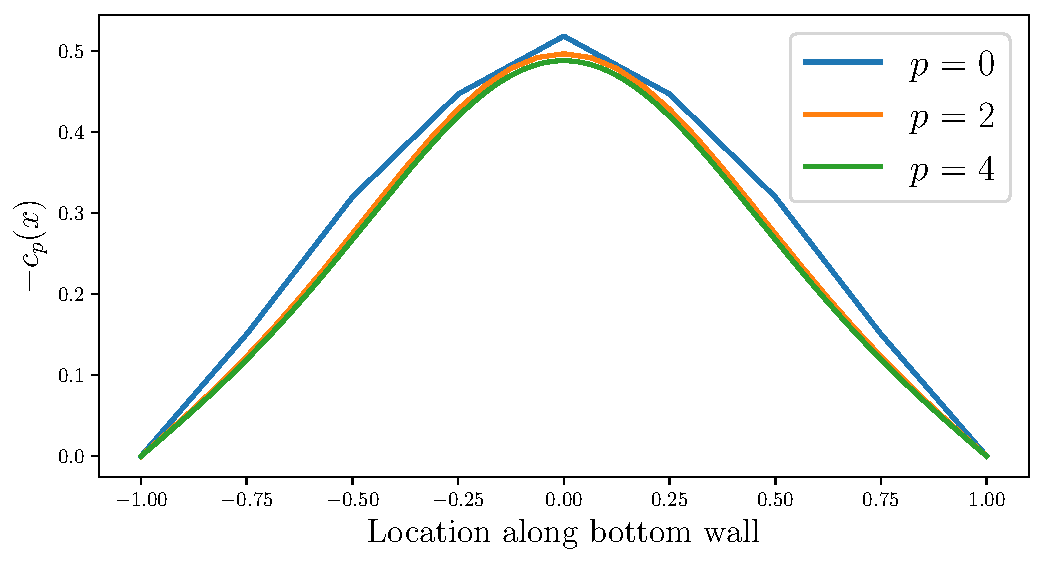
\includegraphics[width = 0.9\linewidth]{tasks/figs/cp_runs.pdf}
    \caption[Coefficient of Pressure Along Bottom Wall.]{P-scaling coefficient of pressure $-c_p(x)$ along bottom wall.}
    \label{fig:cp_runs}
\end{figure}

Looking above to Figure \ref{fig:cp_runs}, increasing $p$ will simply ``\textit{smooth}'' out the coefficient of pressure as it varies along $x$. Notable is that $-c_p(x)$ increases as it gets to the middle, where the middle of the square lies about the $x$-axis. This increase in $-c_p(x)$ indicates that the flow is increasing here as the coefficient of pressure indicates how the local flow is changing with respect to the ambient flow $U_\infty$.

\medskip
Nextly, after having approximated $u$, is to solve for the coefficient of lift $c_l$ using Equation \ref{eqn:cl}. However, to approximate this integral I will use the trapezoidal integration method shown below in Equation \ref{eqn:trapz}.

\begin{equation}
    \int_a^bf(x)\ dx \approx \frac{\Delta x}{2}\left(f(x_N) + f(x_0)\right) + \Delta x\sum_{i=0}^N f(x_i)
    \label{eqn:trapz}
\end{equation}\myequations{Expression For Trapazoidal Integration}

\pagebreak
Using Equation \ref{eqn:trapz} to numerically approximate the coefficient of lift through Equation \ref{eqn:cl}, I can approximate the coefficient of lift per specific $p$ value. Through this method I will run a simulation with $p=7$ to approximate an ``\textit{exact}'' solution. Using this method I get the following results in Table \ref{tab:cl_vals} below.

\begin{table}[h]
    \centering
    \caption{Coefficient of lift $c_l$ values at $p$.}
    \label{tab:cl_vals}
    \begin{tabular}{c | c}
        $p$ & $c_l$\\
        \hline\hline
        \input{tasks/cl_vals}
    \end{tabular}
\end{table}

Conducting this simulation again with $p=7$ approximates the ``\textit{exact}'' solution to be,
\begin{equation*}
    \boxed{c_{l,exact}(p=7) = \input{tasks/cl_exact}}
\end{equation*}

Using this value to be the exact solution, I can then approximate the convergence rate of the simulations by taking the absolute value of the difference and comparing it to the $p$ value and obtaining the rate of convergence as $r = \frac{\log_{10}{\tau_{i+1}/\tau_i}}{\log_{10}{\Delta h_{i+1}/\Delta h_i}}$. Conducting this convergence study gives that the approximated error is,

\begin{figure}[h]
    \centering
    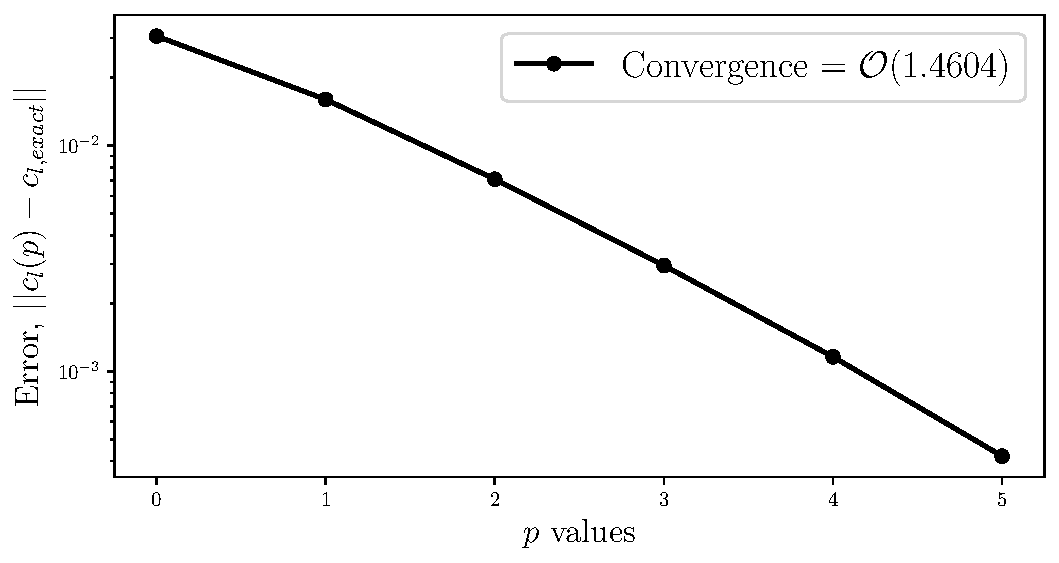
\includegraphics[width = 0.9\linewidth]{tasks/figs/cl_err.pdf}
    \caption[Approximated Residual Error]{Approximated error and convergence while varying $p$.}
    \label{fig:cl_err}
\end{figure}

\begin{fminipage}{0.9\linewidth}
    \textbf{Looking above to Figure \ref{fig:cl_err} the slope of the convergence is $\bf \mathcal{O}(\Delta h^2)$ hence second-order accuracy. This order of accuracy is consistent with the second-oder one-sided finite difference and the 5-point stencil and is the expected slope. This graph confirms the order of accuracy.}
\end{fminipage}